\documentclass[11pt]{beamer}
\usetheme{Madrid}
\usepackage[utf8]{inputenc}
\usepackage{amsmath, amssymb, amsfonts, amsthm}
\usepackage{xcolor}

\usepackage{tikz-cd}

\author[\texttt{sebastiano.tronto@uni.lu}]{Sebastiano Tronto}
\title{Latex Fundamentals}
\logo{
\includegraphics[scale=0.1]{img/unilu.jpg}} 
%\institute{University of Luxembourg} 

\newcommand{\bs}{\textbackslash}

\date{2021-02-19} 

\begin{document}

\begin{frame}
  \titlepage
\end{frame}

\begin{frame}{Latex}
  \begin{enumerate}
    \item Write code (like HTML, not like Python)
    \item Compile to get a pdf file
    \item ???
    \item Profit
  \end{enumerate}
\end{frame}


\begin{frame}{Document structure}
  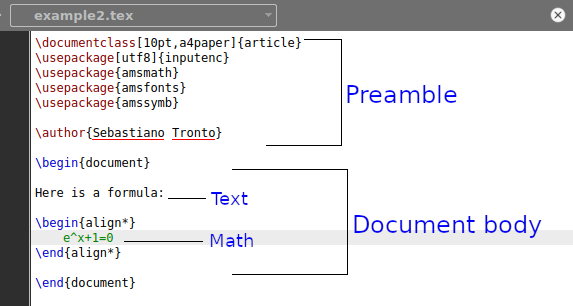
\includegraphics[scale=0.5]{img/example2-preamble-edited.png}
\end{frame}

\begin{frame}{Preamble}
  \begin{itemize}
    \item Include packages with \texttt{\bs usepackage}
    \item Define properties of the document (\texttt{\bs documentclass},
          \texttt{\bs author}, ...)
    \item Define new commands and environments
  \end{itemize}
\end{frame}

\begin{frame}{Text formatting}
  \begin{center}

    \begin{tabular}{ccc}
      \texttt{\small \bs textbf\{Hello\}} &
      \texttt{\small \bs textit\{Hello\}} or \texttt{\small\bs emph\{Hello\}} &
      \texttt{\small \bs underline\{Hello\}} \\
      \textbf{Hello} & \textit{Hello} & \underline{Hello}
    \end{tabular}
  
    \vspace{0.7cm}
      \begin{tabular}{ccc}
      \texttt{\small \{\bs small Hello\}} & \hspace{1cm}
      \texttt{\small \{\bs Large Hello\}} \hspace{1cm} &
      \texttt{\small \{\bs huge Hello\}} \\
      {\small Hello} & {\Large Hello} & {\huge Hello}
    \end{tabular}

  \end{center}
\end{frame}

\begin{frame}{Text formatting}
  Some technicalities:
  \begin{itemize}
    \item Blocks are delimited by \{ and \}
    \item \texttt{\bs textbf\{...\}} etc. are commands with one argument
    \item \texttt{\bs emph\{...\}} is context-aware (when in doubt use this)
    \item \texttt{\bs Large} etc. change the text until the end of the block
    \item Some people use \texttt{\{\bs bf Hello\}}, but it is deprecated
  \end{itemize}
\end{frame}

\begin{frame}{Text formatting}
  \begin{center}
    \begin{tabular}{lc}
      \texttt{\{\bs tiny Hello\}}         & {\tiny Hello} \\
      \texttt{\{\bs scriptsize Hello\}}   & {\scriptsize Hello} \\
      \texttt{\{\bs footnotesize Hello\}} & {\footnotesize Hello} \\
      \texttt{\{\bs normalsize Hello\}}   & {\normalsize Hello} \\
      \texttt{\{\bs large Hello\}}        & {\large Hello} \\
      \texttt{\{\bs Large Hello\}}        & {\Large Hello} \\
      \texttt{\{\bs LARGE Hello\}}        & {\LARGE Hello} \\
      \texttt{\{\bs huge Hello\}}         & {\huge Hello} \\
      \texttt{\{\bs Huge Hello\}}         & {\Huge Hello} \\
    \end{tabular}
  \end{center}
\end{frame}

\begin{frame}{Math mode}
  \texttt{One can write math inline, like
          {\color{red}\bs(} \bs sum\_i\bs frac\{i\}\{2\} {\color{red}\bs)},
          or in displaystyle:
          {\color{red}\bs[} \bs sum\_i\bs frac\{i\}\{2\} {\color{red}\bs]}
         }

  \vspace{1.5cm}
  One can write math inline, like \(\sum_i\frac{i}{2}\) or in displaystyle:
  \[\sum_i\frac{i}{2}\]
\end{frame}

\begin{frame}{Math mode}
  \begin{center}
    For formulas spanning multiple lines you can use:

    \vspace{0.5cm}
    \texttt{\color{red}\bs begin\{align\} (...) \bs end \{align\}}
    \begin{align}
      e^x =& \sum_{n=0}^{\infty} \frac{x^n}{n!} \\
          =& 1 + x + \frac{x^2}{2} + \frac{x^3}{6} + \cdots
    \end{align}
    or \texttt{\color{red}\bs begin\{align*\} (...) \bs end\{align*\}} for no
    numbers.
  \end{center}
\end{frame}

\begin{frame}{Math mode}
  \begin{itemize}
    \item Some people use \texttt{\$2+2=4\$} instead of \texttt{\bs(2+2=4\bs)}
    \item Some \textbf{evil} people use \texttt{\$\$2+2=4\$\$} instead of
          \texttt{\bs[2+2=4\bs]} (don't try this at home!)
    \item For \texttt{align} use \texttt{\bs nonumber} to remove one number
          and \texttt{\&} to align.
    \item For example I always use \texttt{\$2+2=4\$} and the \texttt{align*}
          environment.
  \end{itemize}
\end{frame}

\begin{frame}{Math mode}
  \begin{itemize}
    \item Simple symbols: letters, numbers, $+,-,=,<,>$...
    \item Symbols that need a \textbf{command}:

          \vspace{0.6cm}
          \begin{tabular}{c|c|c|c|c}
            \texttt{\bs alpha, \bs Phi} & \texttt{\bs times, \bs cdot} &
            \texttt{\bs sum} & \texttt{\bs leq, \bs geq} & \texttt{\bs infty}\\
            $\alpha,\Phi$ & $\times,\cdot$ & $\sum$ & $\leq,\geq$ & $\infty$
          \end{tabular}
          \vspace{0.6cm}
    \item Negate symbols with \texttt{\bs not}:
          \begin{align*}
            \texttt{x \bs not \bs in A} \qquad\to&\qquad x\not\in A\\
            \texttt{x \bs not = y}\quad\text{ or }\quad\texttt{x \bs neq y}
             \qquad\to&\qquad x\neq y\\
          \end{align*}
  \end{itemize}
\end{frame}

\begin{frame}{Math mode}
  \begin{itemize}
    \item Some commands take one or more \textbf{arguments} (like 
          \texttt{\bs frac}).
          
          Anything can be an argument:
          \begin{align*}
            \texttt{\bs frac\{1\}\{\bs sum\_\{n\}\}}\qquad\to\qquad
            \frac{1}{\sum_{n} \sqrt n}
          \end{align*}
    \item A few commands take \textbf{options}:
          \texttt{\bs sqrt[3]\{x\}} $\to\,\sqrt[3]{x}$
    %\item Most of these commands work only in Math mode
  \end{itemize}
\end{frame}


\begin{frame}{Math mode}
  \begin{itemize}
    \item Every symbol can have a \textbf{subscript} and a \textbf{superscript}
          \begin{align*}
            \texttt{x\_0\^{}\{23\}} \qquad \to \qquad x_0^{23}
          \end{align*}
    \item Anything can be a sub/superscript:
          \begin{align*}
            \texttt{\bs int\_\{\bs phi (y)\}\^{}\{2\^{}\{n\_1\}\}}
            \qquad \to \qquad \int_{\phi(y)}^{2^{n_1}}
          \end{align*}
  \end{itemize}
\end{frame}


\begin{frame}{Math mode}
  \begin{itemize}
    \item Adjust parentheses size with \texttt{\bs left(} and
          \texttt{\bs right)}: \[\left(\frac{x+6}{y-2}\right)\]
    \item Insert text with \texttt{\bs text} and
          spaces with \texttt{\bs ,} and \texttt{\bs quad}:
          \[\text{this symbol}\quad \sum_{n=0}^\infty \frac{x^n}{n!} \quad
            \text{is in math mode}, this is not text\]
  \end{itemize}
\end{frame}

\begin{frame}{Math mode}
  
  \begin{itemize}
    \item Fancy letters with \texttt{\bs mathcal},
          \texttt{\bs mathbb} and \texttt{\bs mathfrak}:
          \begin{align*}
            \mathcal{A} \qquad \mathbb R \qquad \mathfrak p
          \end{align*}
    \item For custom operators use \texttt{\bs operatorname\{oper\}}:
          \begin{align*}
            \operatorname{oper}(x)
          \end{align*}
    \item Pro-tip: write \texttt{\bs newcommand\{\bs R\}\{\bs mathbb R\}} and
          \texttt{\bs DeclareMathOperator\{\bs lcm\}\{lcm\}} in your preamble!
  \end{itemize}
\end{frame}

\begin{frame}{Math mode}
  \begin{itemize}
    \item Wikibooks page on Math mode:
         {\small\url{https://en.wikibooks.org/wiki/LaTeX/Mathematics}}
    \item Advanced stuff:
         {\small\url{https://en.wikibooks.org/wiki/LaTeX/Advanced_Mathematics}}
    \item List of Mathematical symbols:
         {\small\url{https://www.caam.rice.edu/~heinken/latex/symbols.pdf}}
  \end{itemize}
\end{frame}

\begin{frame}{Environments}
  \texttt{\color{red}\bs begin\{something\}}
    Inside an environment 
  \texttt{\color{red}\bs end\{something\}}

  \vspace{0.8cm}
  \begin{itemize}
    \item We have seen \texttt{document} and \texttt{align}
    \item Text and symbols appear differently depending on the environment
    \item Certain commands are specific to an environment
    \item You can define new environments
  \end{itemize}
\end{frame}


\begin{frame}{Environments}
  Lists: \texttt{\color{red}itemize} and \texttt{\color{red}enumerate}

  \vspace{0.8cm}
  \begin{columns}
    \column{0.5\textwidth}
      \begin{itemize}
        \item First: \[2+2=4\]
        \item Second
      \end{itemize}

    \column{0.5\textwidth}
      \texttt{\bs begin\{itemize\}}

      \texttt{\qquad \bs item First: \bs[2+2=4\bs]}

      \texttt{\qquad \bs item Second}

      \texttt{\bs end\{itemize\}}
  \end{columns}
\end{frame}

\begin{frame}{Environments}
  Tables: \texttt{tabular} (text) and \texttt{array} (Math mode)

  \vspace{0.8cm}
  \begin{columns}
    \column{0.5\textwidth}
      \begin{tabular}{r|cc}
        This & is & just \\
        \hline
          a  & boring & table
      \end{tabular}

    \column{0.5\textwidth}
      \texttt{\bs begin\{tabular\}\{r|cc\}}

      \texttt{\qquad This \& is \& just \bs\bs}

      \texttt{\qquad \bs hline}

      \texttt{\qquad a \& boring \& table}

      \texttt{\bs end\{tabular\}}
  \end{columns}
  
  \vspace{0.8cm}
  Matrices: \texttt{array} with parentheses or \texttt{pmatrix}
\end{frame}

\begin{frame}{Sections}
  \begin{itemize}
    \item Use \texttt{\bs section\{Section Name\}} to start a new section
    \item Also: \texttt{\bs chapter} (book only), \texttt{\bs subsection},
          \texttt{subsubsection}...
    \item \texttt{\bs section*\{Name\}} for no number
    \item Sections after \texttt{\bs appendix} are numbered differently
  \end{itemize}
\end{frame}

\begin{frame}{Theorems}
  
  \begin{itemize}
    \item In preamble: \texttt{\bs usepackage\{amsthm\}}
    \item Also in preamble \texttt{\bs newtheorem \{envname\}\{Theorem\}}
    \item Use \texttt{\bs newtheorem*} for no number
  \end{itemize}
\end{frame}

\begin{frame}{Theorems}
  \begin{columns}
    \column{0.5\textwidth}
      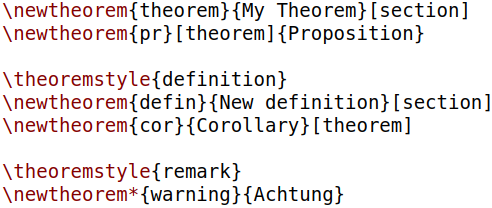
\includegraphics[scale=0.3]{img/thm_pre.png}

      \vspace{0.2cm}
      \vdots
      \vspace{0.3cm}

      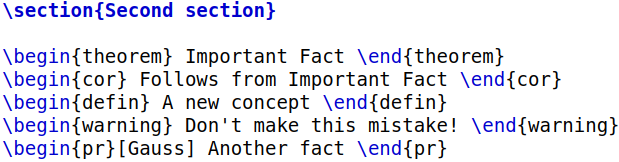
\includegraphics[scale=0.3]{img/thm_tex.png}

    \column{0.5\textwidth}
      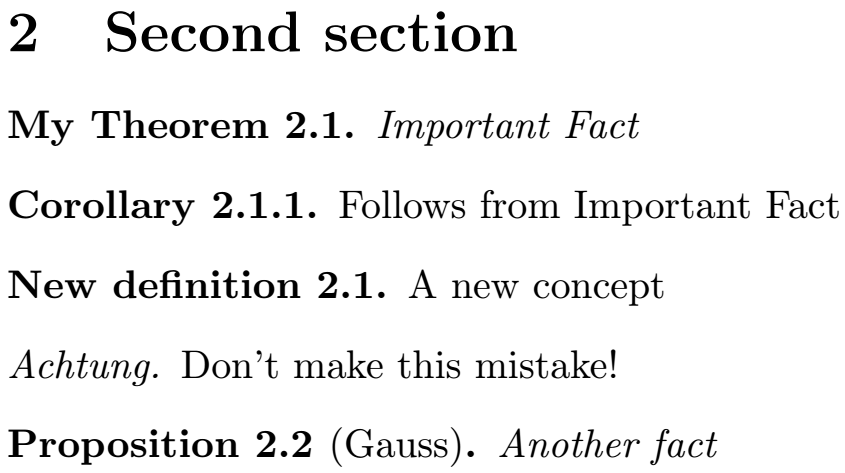
\includegraphics[scale=0.2]{img/thm_pdf.png}

      \vspace{1cm}
  \end{columns}
\end{frame}

\begin{frame}{End of the lecture}
  For next time:

  \vspace{0.8cm}
  \begin{itemize}
    \item Install Latex on your PC
    \item Start writing something in Latex (e.g. homework)
    \item Email me if you have any question
  \end{itemize}
\end{frame}

\end{document}

